\subsection{Nelder-Mead}

\begin{frame}
  \frametitle{Nelder-Mead}

  Метод оптимизации функций без ограничений. 
  
  Поиск экстремальной точки происходит путем операций по изменению симплекса.

  Алгоритм:
  \begin{enumerate}
    \item Сортировка вершин по значению функции в них. Определение $f_h$, $f_s$, $f_l$.
    \begin{align*}
      f_h = \max_j f_j, \quad f_s = \max_{j \neq h} f_j, \quad f_l = \min_{j \neq h, j\neq s} f_j
    \end{align*}

    \item Вычисление центроида без $x_h$
    \begin{equation*}
      c = \frac{\sum_{i \neq h}^{n+1} x_i}{n}
    \end{equation*}
    \item Трансформация симплекса.
  \end{enumerate}


\end{frame}

\begin{frame}
  \frametitle{Трансформации}
  \begin{itemize}
    \item reflection 

      $x_r = c + \alpha(c - x_h)$, если $f_l \leq f_r \leq f_s$, то меняем $x_h$ на $x_r$.
      \begin{figure}
      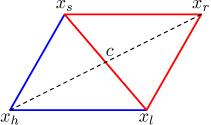
\includegraphics[height=2cm]{figures/reflection.jpg}
      \end{figure}

    \item expansion

    если $f_r < f_l$ то вычисляем $x_e = c + \gamma(x_r - c)$, если $f_e < f_r$, то меняем $x_h$ на $x_e$, иначе на $x_r$.
      \begin{figure}
      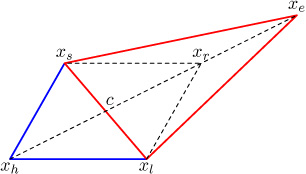
\includegraphics[height=2cm]{figures/expansion.jpg}
      \end{figure}

  \end{itemize}
\end{frame}

\begin{frame}
  \frametitle{Трансформации}
  \begin{itemize}
     \item Contraction

    при $f_r \geq f_l$ вычисляем $x_c$ используя меньшую из $f_r, f_h$ точку.

    $f_r < f_h$: $x_c = c + \beta(x_r - c)$, если  $f_c \leq f_r$ принимаем $x_c$ иначе shrink.

    $f_r \geq f_h$: $x_c = c + \beta(x_h - c)$, если  $f_c < f_h$ принимаем $x_c$ иначе shrink.

  \begin{figure}
    \begin{minipage}{0.4\textwidth}
      \centering
      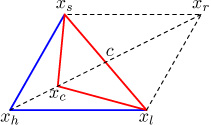
\includegraphics[height=2cm]{figures/contraction2.jpg}
    \end{minipage}
    \begin{minipage}{0.4\textwidth}
      \centering
      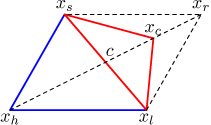
\includegraphics[height=2cm]{figures/contraction1.jpg}
    \end{minipage}
  \end{figure}
  \item Shrink

  Вычисляются n новых вершин симплекса : $x_j := x_l + \delta (x_j - x_l)$
       \begin{figure}
      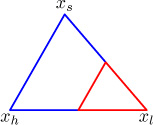
\includegraphics[height=2cm]{figures/shrink.jpg}
      \end{figure}
  
  \end{itemize}
\end{frame}


\begin{frame}
  \frametitle{Выбор начального симплекса}
  \begin{itemize}
    \item Выбирается начальное приближение экстремальной точки $x_0$.

    \begin{equation*}
      x_j = x_0 + h_j e_j,
    \end{equation*}

  $e_j$ -- направление, $h_j$ -- длина шага в направлении.


  \item Авторы оригинальной статьи предлагают строить правильный симплекс с одной из вершин в $x_0$.
\end{itemize}
\end{frame}
